\documentclass{article}
\usepackage{graphicx}
\usepackage[brazil]{babel}
\usepackage[utf8]{inputenc}

\begin{document}

\title{Closeness Vitality - Implementação Individual, da Disciplina SCC5882}
\author{Renato Fabbri}

\maketitle

\begin{abstract}
Este documento descreve a implementação da medida \emph{Closeness Centrality}. Uma breve introdução ao conceito da medida é seguido por uma descrição mais formal e a apresentação do algoritmo em si. Há uma figura ilustrativa do resultado e uma discussão do resultado encerra o documento. Junto a este documento deve se encontrar o algoritmo em Python que realiza a medida para um vértice específico ou para uma aresta específica. Também há na implementação as linhas necessárias para a realização da visualização gráfica da medida e para calcular a medida para todos os vértices ou todas as arestas de um grafo.
\end{abstract}

\section{Sobre a Medida Closeness Vitality}
Intuitivamente uma medida de centralidade realizada em um grafo ou rede complexa é uma medida da importância que tem o elemento (seja ele um vértice ou uma aresta). Uma requisição mínima que comumente se impõe a uma medida de centralidade é que ela dependa somente da estrutura do grafo.

Uma definição mais formal de índice de centralidade pode ser dada utilizando a noção de índice estrutural. Um índice estrutural é uma medida que permanece a mesma entre elementos correspondentes de grafos isomorfos.

As primeiras medidas de centralidade foram introduzidas na década de 50. Visto que nem toda medida de centralidade é propícia para toda aplicação, várias medidas foram desenvolvidas desde então.

Este documento descreve a medida chamada \emph{Closeness Vitality} e sua implementação. A medida closeness vitality é baseada no Índice de Werner de um Grafo $G$, $I_W(G)$ definido assim:

\begin{equation}
    I_W(G) = \sum_{v \in V}\sum_{w \in V}d(v,w)
\end{equation}

Onde $d(v,w)$ é a menor distância entre os vértices $v$ e $w$. Ou seja, $I_W(G)$ é a soma das (menores) distâncias entre todos os pares de vértices.

A medida de centralidade comumente chamada closeness vitality, denotada $c_{CV})$ é definida da seguinte forma:

\begin{equation}
    c_{CV} = I_W(G) - I_W(G\backslash{x})
\end{equation}

Este índice mede o custo de transporte entre os pares de vértice caso o vértice de referência da medição seja removido.

Claramente, esta medida pode ser feita para uma aresta ao invés de um vértice. A fórmula e raciocínio é exatamente o mesmo: o custo de comunicação/transporte envolvido em se retirar a aresta.

\section{Implementação}
A implementação em \emph{closeness\_vitality.py} calcula o índice de closeness vitality para qualquer vértice ou aresta do grafo dado. Também pode lidar com grafos com ou sem peso, dirigidos ou não. A forma como o código está escrito permite sua utilização como uma função ordinária do Python ou de qualquer biblioteca externa. Também foi feito uma pequena demostração gráfica na qual o script calcula o índice para todos os nós e plota um gráfico com uma coloração para cada nó que reflete o valor do índice closeness vitality do nó.

Para utilizá-la como função padrão, basta:

\begin{verbatim}
    >>> from closeness_vitality import *
    >>> cv = closeness_vitality(g, v) # g um grafo do networkx e v um vértices
\end{verbatim}

Para rodar a demonstração que calcula o índice para todos os nós e plota o grafo com cores correspondentes aos valores dos índices (com uma barra de cor para que se tenha referência), basta rodar:

\begin{verbatim}
    $ python closeness_vitality.py
\end{verbatim}


\subsection{Conclusão e Resultados}
Ao final do documento está o gráfico exibido pelo script desenvolvido para este trabalho.

Note que os vértices periféricos tem valor positivo, ou seja, caso sejam removidos, diminuem a distância geral entre cada par de vértices, pois não são atalho para praticamente ninguém e estão longe de quase todos. Já os vértices centrais claramente exibem valores que refletem sua importância para o encurtamento das distâncias entre os demais vértices.

A medida pode ser utilizada para diversas aplicações, em especial para avaliar sistemas que envolvam transporte e comunicação.

Também vale apontar que a implementação realizada pode ser utilizada em grafos com construções diferentes (dirigidos ou não diridos, com ou sem peso) e que pode ser utilizada como um função Python qualquer, com facilidade de aproveitamento em projetos específicos.


\begin{figure}
    \centering
    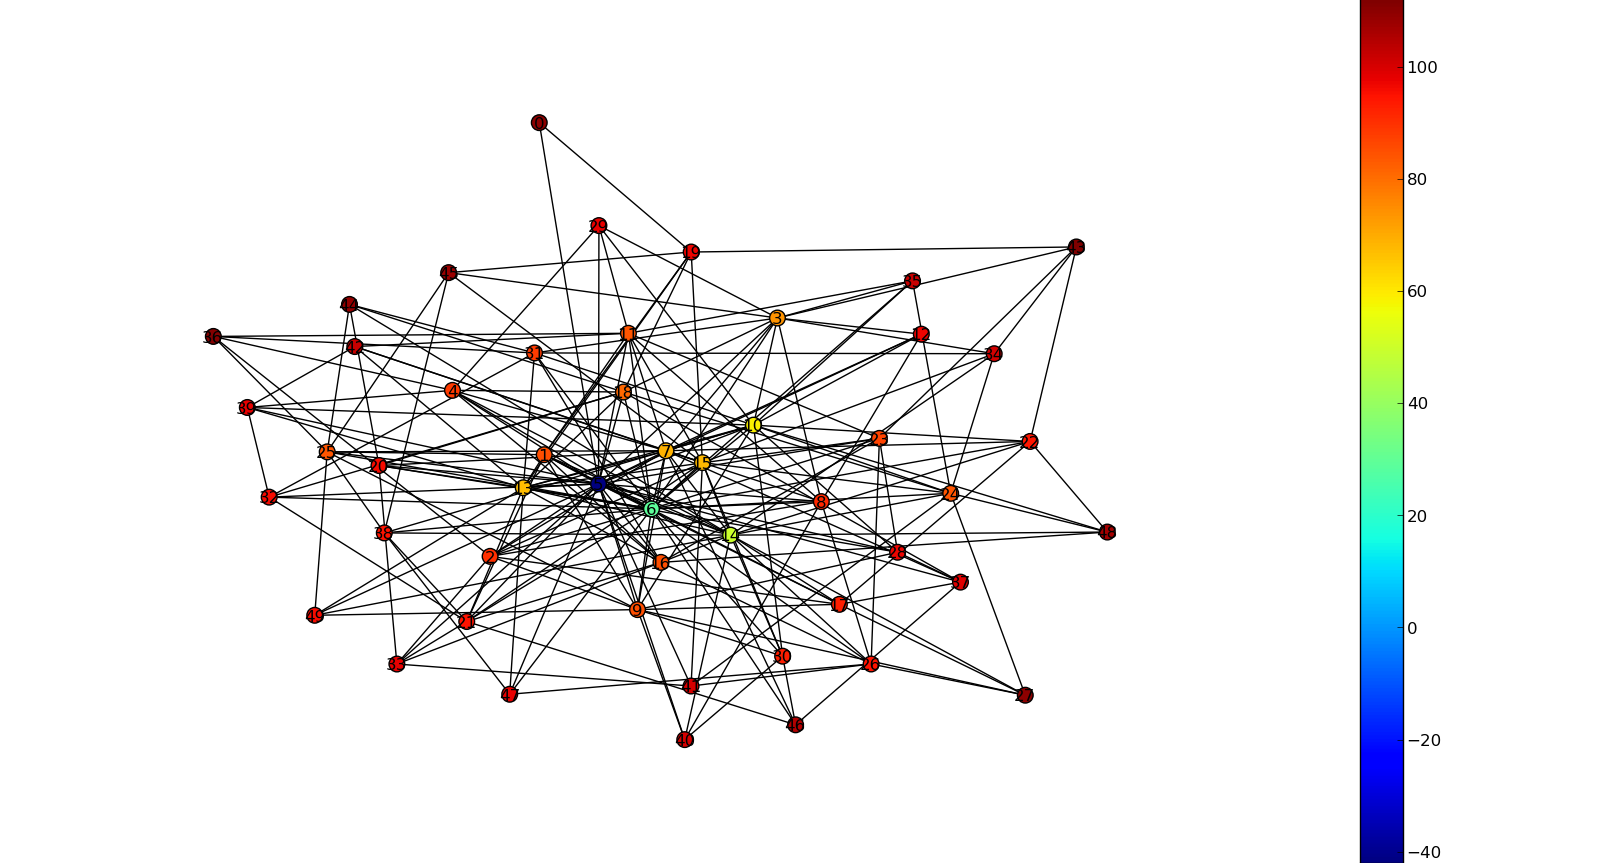
\includegraphics[width=6.0in]{rede-plotada}
    \caption{Índices de Closeness Vitality para cada Nó, conforme demo do script}
    \label{simulationfigure}
\end{figure}


\begin{thebibliography}

\bibitem{nx}Ulrik Brandes and Thomas Erlebach , \textsl{Network Analysis: Methodological Foundations},
Springer; 1 edition, 2005.

\bibitem{nx}Aric Hagberg, Dan Schult, and Pieter Swart and Others, \textsl{networkx: High productivity software for complex networks},
http://networkx.lanl.gov/.



\end{thebibliography}

\end{document}

